\documentclass{beamer}

\usepackage{style}


\title[Hex]{Le Dévelopement d'un programme joueur}
\date{T.I.P.E 2015--2016}
\subject{Informatiques et Mathématiques}

\begin{document}

\begin{frame}
  \titlepage
\end{frame}

\begin{frame}
  
\includegraphics[scale=0.5]{img/AlphaGo}
\end{frame}

\begin{frame}
  \frametitle{Plan}
  \tableofcontents[hideallsubsections]
\end{frame}

\section{Introduction}

\begin{frame}
  \frametitle{Hex}
  \begin{HexBoard}[board size=10]
  \end{HexBoard}
\end{frame}

\section{Aproche simple}

\subsection{Présentation}
\begin{frame}
  \frametitle{Présentation de l'algorithme Minimax}
  % vim: ft=tex

\begin{tikzpicture}
    \tikzstyle{solid node}=[circle,draw,inner sep=1.5,fill=black]
    \tikzstyle{level 1}=[level distance=20mm,sibling distance=40mm]
    \tikzstyle{level 2}=[level distance=20mm, sibling distance=20mm]
    \node(0)[solid node, label=above:{Noir}]{}
        child{node(1)[solid node]{}
            child{node(2)[solid node, label=below:{N}]{}}
            child{node(3)[solid node, label=below:{B}]{}}
        }
        child{node(4)[solid node]{}
            child{node(5)[solid node, label=below:{N}]{}}
            child{node(6)[solid node, label=below:{N}]{}}
        }
        child{node(7){} edge from parent[dashed]};
    \draw[dashed,rounded corners=7]
        ($(1)+(-.25,.25)$)rectangle($(4)+(.25,-.25)$);
    \node at($(1)!.5!(4)$){Blanc};
    \node[left,visible on=<2->,xshift=-5] at(1){B};
    \node[right,visible on=<2->,xshift=5] at(4){N};
\end{tikzpicture}

\end{frame}


\subsection{Complexité}
\newcommand{\game}{
  \HStoneGroup[color=white]{
    a3,a5,b1,b4,b5,c1,c2,d4,d5,e1,e2,e5,c3}
  \HStoneGroup[color=black]{
    a2,a4,b2,b3,c4,c5,d1,d2,d3,e3,e4,a1}
}

\begin{frame}
  \frametitle{Décomposition du minimax}
  \begin{itemize}
    \item \func{getWinningPlay}
    \item \func{winner}
  \end{itemize}
\end{frame}

\subsubsection{\func{winner}}

\newcommand{\hexGameProcessOnBlack}[2]{
  \begin{HexBoard}[board size=5]
    \game{}
    \HStoneGroup[color=black,label=\verifier]{#1}
    \HStoneGroup[color=black,label=\estVerifier]{#2}
  \end{HexBoard}
}

\newcommand{\hexWorstCase}{
    \begin{HexBoard}[board size=5,hex height=0.5cm]
      \HStoneGroup[color=black]{
        a1,a2,a3,a4,a5,b1,b2,b3,b4,b5,c1,c2}
      \HStoneGroup[color=white]{
        c3,c4,c5,d1,d2,d3,d4,d5,e1,e2,e3,e4,e5}
    \end{HexBoard}
}

\newcommand{\verifier}{\stoneMark{V}}
\newcommand{\estVerifier}{\stoneMark{A}}

\begin{frame}
  \frametitle{\func{winner}}
  \begin{HexBoard}[board size=5]
    \game{}
  \end{HexBoard}
\end{frame}

\begin{frame}
  \frametitle{Implémentation}
  \hexGameProcessOnBlack{d1}{d2}
\end{frame}

\begin{frame}
  \frametitle{Implémentation}
  \hexGameProcessOnBlack{d1,d2}{d3}
\end{frame}

\begin{frame}
  \frametitle{Implémentation}
  \hexGameProcessOnBlack{d1,d2,d3}{e3}
\end{frame}

\begin{frame}
  \frametitle{Implémentation}
  \hexGameProcessOnBlack{d1,d2,d3,e3}{e4}
\end{frame}

\begin{frame}
  \frametitle{Implémentation}
  \hexGameProcessOnBlack{d1,d2,d3,e3,e4}{c4}
\end{frame}

\begin{frame}
  \frametitle{Implémentation}
  \hexGameProcessOnBlack{d1,d2,d3,e3,e4,c4}{c5}
\end{frame}

\begin{frame}
  \frametitle{Calcul de la compléxité}
  \begin{columns}
    \begin{column}{5cm}
      \hexWorstCase
    \end{column}
    \begin{column}{5cm}
    \begin{itemize}
      \item Compléxité d'un parcours
      \begin{align*}
        P(n) &= \sum^{\left\lceil\frac{n^2}{2}\right\rceil}_{k = 1} k \\
        \implies P(n) &= O\left(\left\lceil\frac{n^2}{2}\right\rceil^2\right) \\
        \implies P(n) &= O\left(n^4\right)
      \end{align*}
      \item Compléxité de \func{winner}
      \[
        W(n) = n P(n) = O\left(n^5\right)
      \]
    \end{itemize}
    \end{column}
  \end{columns}
\end{frame}


\subsubsection{\func{getWinningPlay}}

\begin{frame}
  \frametitle{\func{getWinninglay}}
  \begin{tikzpicture}
    \tikzstyle{solid node}=[circle,draw,inner sep=1.5,fill=black]
    \tikzstyle{level 1}=[level distance=20mm,sibling distance=40mm]
    \tikzstyle{level 2}=[level distance=20mm, sibling distance=20mm]
    \node(0)[solid node, label=above:{Noir}]{}
        child{node(1)[solid node]{}
            child{node(2)[solid node, label=below:{N}]{}}
            child{node(3)[solid node, label=below:{B}]{}}
        }
        child{node(4)[solid node]{}
            child{node(5)[solid node, label=below:{N}]{}}
            child{node(6)[solid node, label=below:{N}]{}}
        }
        child{node(7){} edge from parent[dashed]};
    \draw[dashed,rounded corners=7]
        ($(1)+(-.25,.25)$)rectangle($(4)+(.25,-.25)$);
    \node at($(1)!.5!(4)$){Blanc};
\end{tikzpicture}

\end{frame}

\begin{frame}
  \frametitle{Calcul de la compléxité}
  \newcommand{\enumeratenode}[1]{
  node{\scriptsize $\cdots #1 \cdots$} 
  edge from parent[draw=none]
}

\newcommand{\winnercomplexity}{\footnotesize $W(n)$}

\begin{tikzpicture}

\tikzstyle{level 2}=[sibling distance=12mm]

\node[draw,circle]{$n^2$}
  child{node[draw,circle]{$n^2$}
    child{node[draw,circle]{$n^2$}
      child{node{$\vdots$}
        child{node[circle,draw]{\winnercomplexity}}
      }
    }
    child{node[draw,circle](g){$n^2$}
      child{node{$\vdots$}
        child{node[circle,draw]{\winnercomplexity}}
      }
    }
    child{\enumeratenode{n^2 - 1}}
    child{node[draw,circle](h){$n^2$}
      child{node{$\vdots$}
        child{node[circle,draw]{\winnercomplexity}}
      }
    }
  }
  child[missing]
  child{node[draw,circle](a){$n^2$}
    child{node{$\vdots$}
      child{node{$\vdots$}
        child{node[circle,draw]{\winnercomplexity}}
      }
    }
  }
  child{\enumeratenode{n^2 - 2}}
  child{node[draw,circle](b){$n^2$}
    child{node{$\vdots$}
      child{node{$\vdots$}
        child{node[circle,draw]{\winnercomplexity}}
      }
    }
  };

\end{tikzpicture}

\end{frame}

\begin{frame}
  \frametitle{Calcul de la compléxité d'un étage}
  Pour le $p$-ème étage.

  \pause

  $p$ coups à jouer parmis $n^2$ cases.

  \pause
  $\mathcal{A}^{n^2}_p$ noeuds
  \pause
  \begin{align*}
    E_p(n) &= \mathcal{A}^{n^2}_p n^2 \\
    \implies E_p(n)  &= \frac{(n^2)!}{(n^2 - p)!} n^2 \\
  \end{align*}
\end{frame}

\begin{frame}
  \frametitle{Calcul de la compléxité total}
  $n^2$ étages.
  \pause
  \[
    M(n) = \sum^{n^2}_{k = 1} E_p(n) + n^2! \; W(n)
  \]
  \pause
  \[
    M(n) = \sum^{n^2}_{k = 1} \left(\frac{(n^2)!}{(n^2 - p)!} n^2\right)
    + n^2! \; O\left(n^5\right)
  \]
  \pause
  \begin{align*}
    M(n) &= O\left(n^2! \; n^4\right) + n^2! \; O\left(n^5\right) \\
    \implies M(n) &= O\left(n^2! \;n^5\right)
  \end{align*}
\end{frame}
  



\section{Recherche aléatoire}

\subsection[Présentation]{Présentation de l'implémentation}
\newcommand{\continuationNode}{
  node[draw=none]{} edge from parent[dashed,thin,-]
}

\newcommand{\rechercheAleatoireOne}{
  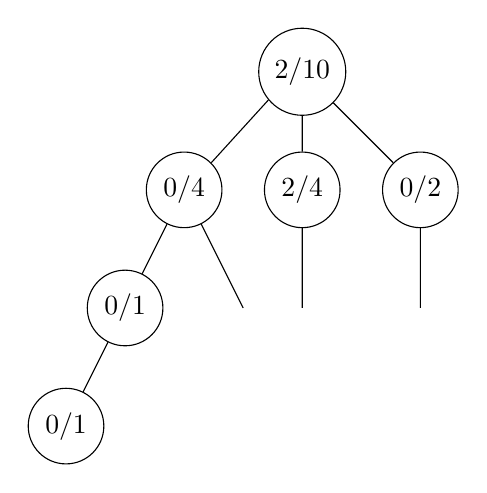
\begin{tikzpicture}[nodes={draw,circle}]
    \node{$2/10$}
      child{node{$0/4$}
        child{node{$0/1$}
          child{node{$0/1$}}
          child[missing]
        }
        child{\continuationNode}
      }
      child{node{$2/4$}
        child{\continuationNode}
      }
      child{node{$0/2$}
        child{\continuationNode}
      };
  \end{tikzpicture}
}

\newcommand{\rechercheAleatoireTwo}{
  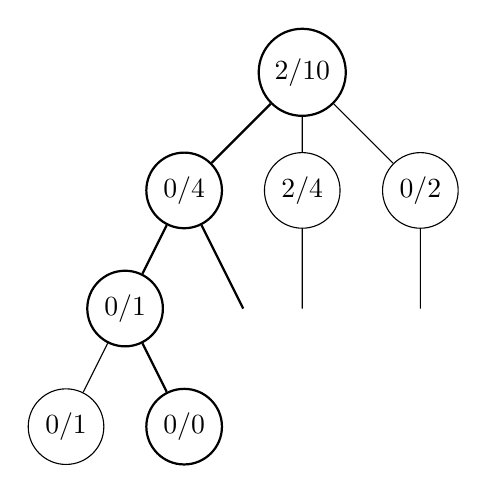
\begin{tikzpicture}[nodes={draw,circle}]
    \node[thick]{$2/10$}
      child{node[thick]{$0/4$}edge from parent[thick]
        child{node[thick]{$0/1$}edge from parent[thick]
          child{node[thin]{$0/1$}edge from parent[thin]}
          child{node[thick]{$\boldsymbol{0/0}$}edge from parent[thick]}
        }
        child{\continuationNode}
      }
      child{node{$2/4$}
        child{\continuationNode}
      }
      child{node{$0/2$}
        child{\continuationNode}
      };
  \end{tikzpicture}
}

\newcommand{\rechercheAleatoireThree}{
  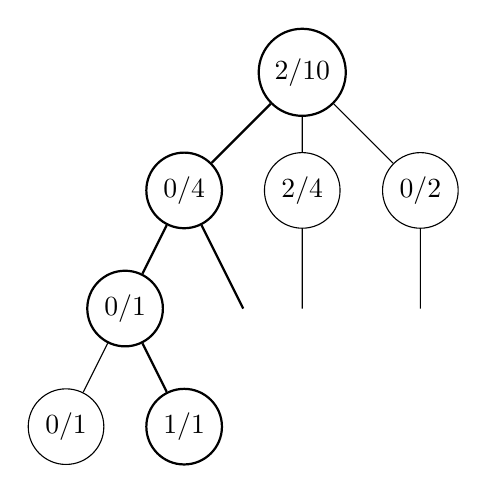
\begin{tikzpicture}[nodes={draw,circle}]
    \node[thick]{$2/10$}
      child{node[thick]{$0/4$}edge from parent[thick]
        child{node[thick]{$0/1$}edge from parent[thick]
          child{node[thin]{$0/1$}edge from parent[thin]}
          child{node[thick]{$\boldsymbol{1/1}$}edge from parent[thick]}
        }
        child{\continuationNode}
      }
      child{node{$2/4$}
        child{\continuationNode}
      }
      child{node{$0/2$}
        child{\continuationNode}
      };
  \end{tikzpicture}
}

\newcommand{\rechercheAleatoireFour}{
  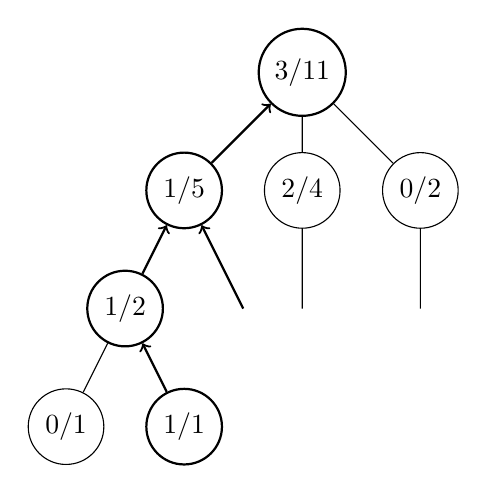
\begin{tikzpicture}[nodes={draw,circle}]
    \node[thick]{$3/11$}
      child{node[thick]{$1/5$}edge from parent[thick,<-]
        child{node[thick]{$1/2$}edge from parent[thick,<-]
          child{node[thin]{$0/1$}edge from parent[thin,-]}
          child{node[thick]{$\boldsymbol{1/1}$}edge from parent[thick,<-]}
        }
        child{\continuationNode}
      }
      child{node{$2/4$}
        child{\continuationNode}
      }
      child{node{$0/2$}
        child{\continuationNode}
      };
  \end{tikzpicture}
}


\begin{frame}
  \frametitle{Représentation sous forme d'arbre}
  \rechercheAleatoireOne
\end{frame}

\begin{frame}
  \frametitle{Représentation sous forme d'arbre}
  \rechercheAleatoireTwo
\end{frame}

\begin{frame}
  \frametitle{Représentation sous forme d'arbre}
  \rechercheAleatoireThree
\end{frame}

\begin{frame}
  \frametitle{Représentation sous forme d'arbre}
  \rechercheAleatoireFour
\end{frame}


\subsection[Différence]{Avantages et inconvenients de la recherche 
  aléatoire}
\begin{frame}
  \frametitle{Avantage}
  \begin{itemize}
    \item<2-> Donne un résultat en un temp fini.
    \item<3-> Peux facilement être utilisé pendant le long d'une partie.
  \end{itemize}
\end{frame}

\begin{frame}
  \frametitle{Inconvénients}
  \begin{itemize}
    \item<2-> Perds la sureté de la victoire.
    \item<3-> Utilise beaucoup mémoire.
  \end{itemize}
\end{frame}


\subsection[Efficacité]{Etude de l'efficacité de l'algorithme de recherche
  aléatoire}

\newcommand{\tempTaille}[1][1.0]{
  \begin{tikzpicture}[scale=#1]
    \begin{semilogyaxis}[
      title=Temp d'un teste en fonction de la taille,
      xlabel={Temp pris par un teste},
      ylabel={Taille du plateau}
    ]
      \addplot[blue] table {data/values_1.dat};
      \addplot[green] table {data/values_5.dat};
      \addplot[red] table {data/values_9.dat};
      \addplot[brown] table {data/values_11.dat};
    \end{semilogyaxis}
  \end{tikzpicture}
}

\newcommand{\tempTailleCarre}[1][1.0]{
  \begin{tikzpicture}[scale=#1]
    \begin{semilogyaxis}[
      title=Temp d'un teste en fonction du carre de la taille,
      xlabel={Temp pris par un teste},
      ylabel={Taille du plateau}
    ]
      \addplot[blue] table {data/temp_pris_test_carre.dat};
    \end{semilogyaxis}
  \end{tikzpicture}
}



\begin{frame}
  \frametitle{Statistique}
  \begin{columns}
    \begin{column}{5cm}
      Mettre ici Nombre de teste en fonction du temp
      \tempTaille[0.6]
    \end{column}
    \begin{column}{5cm}
      Mettre ici Espace utilisé en fonction du temp
    \end{column}
  \end{columns}
\end{frame}




\section{Conclusion}
\begin{frame}
  \frametitle{Amélioration Possible}
  \begin{itemize}
    \item<2-> Structure de donnée adaptée
    \item<3-> Fonction d'évaluation
    \item<4-> Plus d'information sur la partie
  \end{itemize}
\end{frame}



\end{document}
